\documentclass{article}
\usepackage{epsf, a4, makeidx, Manu}
\usepackage{palatino}
\usepackage{multicol}
\usepackage{graphicx} 
\usepackage[utf8]{inputenc}
\usepackage[french]{babel}

\newcommand{\note}[1]{}
\title{La gestion de la mémoire}

\author{Chaput Emmanuel}

\usepackage{listings}
\lstloadlanguages{C}
\lstdefinelanguage{nasm}%
  {keywords={add, call, mov, iret, lcall, ljmp, jmp, push, pop, ret, shl, shr, xor},%
   otherkeywords={eax, ebx, ecx},%
   ndkeywords={ax, bx, cx},%
   sensitive=f,%
   morecomment=[l]{;},%
  }[keywords,comments,strings]%




\begin{document}

\lstset{language=C,%
        basicstyle=\ttfamily,%
        keywordstyle=\bfseries,%
        ndkeywordstyle=\bfseries \underbar ,%
        identifierstyle=\em,%
        extendedchars}


%===============================================================================
%      Gestion de la mémoire
%===============================================================================
\section{Gestion de la mémoire}

   La gestion de la mémoire est une fonction essentielle d'un système
d'exploitation. Nous allons dans un premier temps jeter un coup
d'\oe{}uil rapide à la gestion de la mémoire vue par Intel.

   Il y a plusieurs concepts à intégrer. Cela peut sembler complexe,
mais en prenant un peu de temps, vous vous rendrez compte qu'il n'y a
rien de méchant !

   Le premier est la {\em segmentation}. Pour faire simple,
imaginez-vous fin des années 70 avec un microprocesseur dont les
registres sont sur 32 bits. Comment adresser plus de 64 Ko ? La
segmentation consiste à utiliser deux registres pour composer une
adresse de plus de 32 bits. Nous allons voir que ce concept a été
enrichi et utilisé à d'autres fins.

   Le second est la {\em pagination}. L'idée ici est de découper la
mémoire en {\em pages} de taille fixe. Chaque page pourra être dotée
de propriétées qui lui sont propre. La pagination va nécessiter la
mise en place d'un certain nombre de tables d'indirection, ce qui peut
sembler un peu lourd, mais qui va en particulier permettre de la
mémoire virtuelle, de l'isolation entre les tâches, \ldots

%-------------------------------------------------------------------------------
%
%-------------------------------------------------------------------------------
\subsection{La segmentation}

   Essayons de comprendre ce qui se passe lorsqu'une instruction du
processeur doit manipuler une adresse. Nous nous en tiendrons ici à
l'architecture des Intel 386.
   
   Imaginons par exemple une instruction qui doit aller lire ou écrire
un octet en mémoire ou encore une instruction qui effectue un saut
vers une nouvelle zone de code. Une telle instruction va donc exprimer
explicitement une adresse, appelée {\em adresse logique}. Cette
adresse logique est composée de deux parties : un {\em segment}, et un
{\em offset}.

   Le segment est une partie de la mémoire, et l'offset un déplacement
dans le segment, comme l'illustre la figure \ref{Fig-1}. On
peut donc voir ça comme une découpe de la mémoire 
en zones (ou segments) logiques et/ou comme une façon d'accéder à des
adresses plus élevées que ce que permet la taille des registres.

%\begin{figure}[htbp]
%$$
%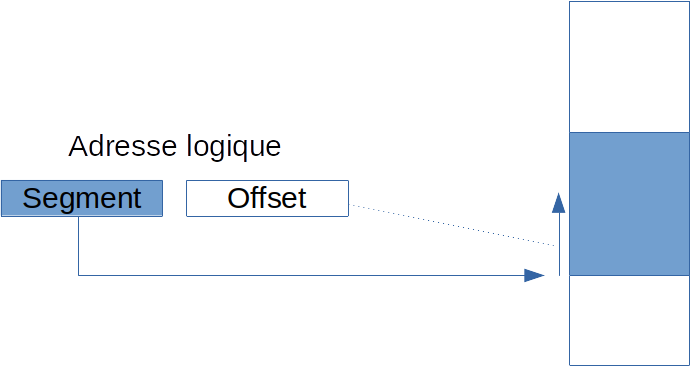
\includegraphics[width=0.4\textwidth]{adresse-logique}
%![](adresse-logique.png){}

\begin{figure}[htbp]
\begin{center}
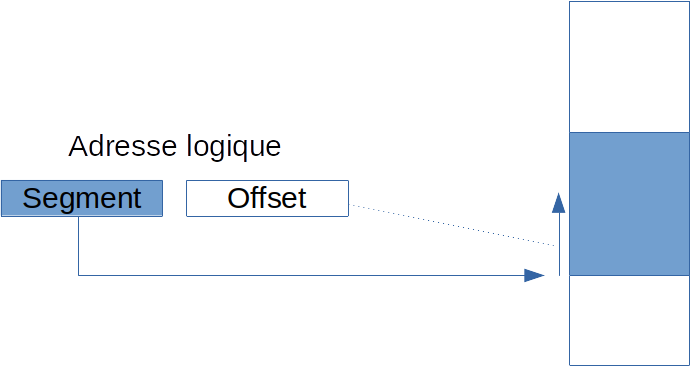
\includegraphics[width=0.6\textwidth]{adresse-logique.png}
\caption{\label{Fig-1}Adresse logique}
\end{center}
\end{figure} 

   Le segment est contenu dans un registre qui peut être fourni
explicitement ou implicitement par l'instruction. Il donne donc
l'adresse de la zone mémoire que l'on appelle un segment. Sauf que
c'est malheureusement un peu plus complexe que ça ! Un segment n'est
en effet pas décrit uniquement par son adresse (et quand bien même !
On a dit qu'un registre ne pouvait pas contenir une adresse entière).

   En fait, le registre en question permet d'accéder à un {\em
descripteur de segment}. C'est évidemment ce dernier (que nous
allons décrire par la suite) qui donne, entre autres, l'adresse du
segment. La figure \ref{Figure:addlogsel} illustre cette indirection.

\note{
\begin{figure}[htbp]
$$
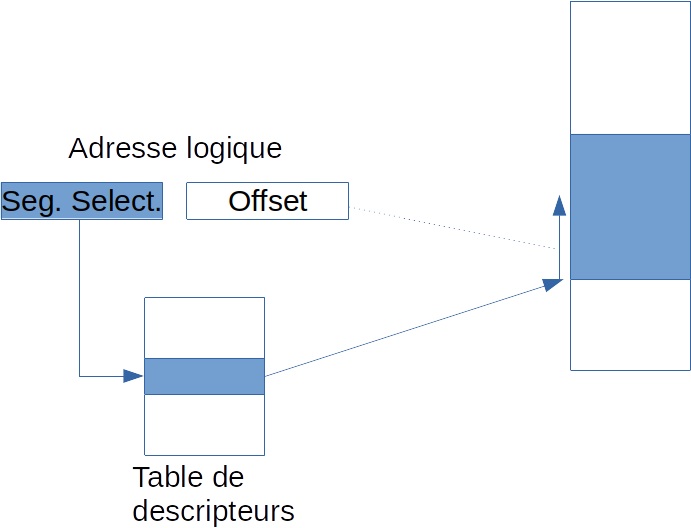
\includegraphics[width=0.4\textwidth]{adresse-logique-sel}
$$
\caption{\label{Figure:addlogsel}Adresse logique et sélecteur de segment}
\end{figure} 
}

%-------------------------------------------------------------------------------
%      Segmentation
%-------------------------------------------------------------------------------
%\subsection{La segmentation sur les processeurs Intel}

   Dans les versions antérieures de ses processeurs (et dans le mode
``réel'' du 386), la mémoire est découpée logiquement en {\em
segments}. Une adresse est alors désignée par un couple composé d'un
{\em registre de segment} et d'un {\em registre d'offset}.

   Concrètement, la taille d'un segment est de 64 Ko (puisque le
registre d'offset est sur 32 bits).

   À partir du 286 (si je ne me trompe pas), en mode dit ``protégé'', un
registre de segment devient une référence vers un {\em descripteur de
segment}. Ce dernier permet une gestion beaucoup plus évoluée de la
mémoire.

   Les descripteurs de segment sont rassemblés dans une table, la {\sc 
gdt} ({\em {\bf G}lobal {\bf D}escriptor {\bf T}able}) ou la {\sc ldt}
({\em {\bf L}ocal {\bf D}escriptor {\bf T}able}). Un registre de
segment représente alors simplement le décalage d'un descripteur dans
la table.

   Lorsque l'on utilise un registre de segment, il contient donc
en fait l'adresse (dans la {\sc ldt} ou dans la {\sc gdt}) d'un
descripteur de registre. Ce descripteur contient lui-même l'adresse du
segment.

%...............................................................................
%      Les descripteurs de segment
%...............................................................................
\subsubsection{Les descripteurs de segment}

   La figure \ref{Figure:DescrSegment} montre la structure d'un
descripteur de segment.

\note{
  \begin{figure}[htbp]
$$
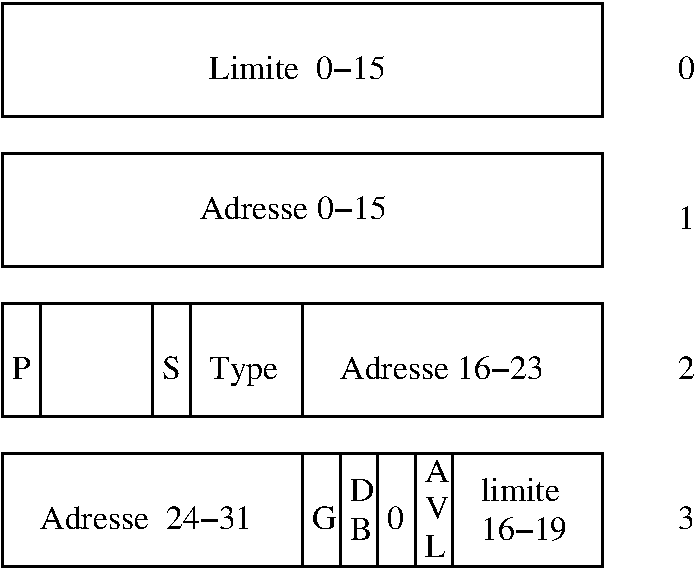
\includegraphics[width=0.3\textwidth]{DescrSegment}
$$
\caption{\label{Figure:DescrSegment}Structure d'un descripteur de segment}
\end{figure} 
}
   Dans ManuX, la fonction suivante crée un descripteur de segment et
l'ajoute dans la {\sc gdt} ou la {\sc ldt} passée en paramètre :

\begin{lstlisting}{}
int setDescripteurSegment(DescriptorTable * dt,
                          uint32 adresse, uint32 limite,
                          uint8 type,
                          uint8 gd0a)
\end{lstlisting}  

   Pour cela, elle initalise une structure de type
\lstinline!DescSegment! définie dans
\lstinline!include/i386/segment.h! de la façon suivante

\begin{lstlisting}{}
typedef struct _DescSegment {
   uint16 limiteFaible;
   uint16 baseFaible;
   uint8  baseInter;
   uint8  type;
   uint8  limiteFort;
   uint8  baseFort;
} DescSegment;
\end{lstlisting}  

%...............................................................................
%      Les LDT et la GDT
%...............................................................................
\subsubsection{Les tables de descripteurs de segments {\sc ldt} et {\sc gdt}}

   La {\sc gdt} est donc la table globale contenant les descripteurs
de segment du système.

   Dans ManuX, elle est initialisée par la fonction suivante

\begin{lstlisting}{}
void initialiserGDT();     
\end{lstlisting}

   Pour le moment, cette fonction est la plus simple possible, elle
crée quatre descripteurs de segments

\begin{itemize}
   \item un descripteur nul, obligatoire ;
   \item un descripteur pour le segment de code, occupant les 4 Go de base ;
   \item un descripteur pour le segment de données, occupant les 4 Go de base ;
   \item un descripteur pour le segment de pile, occupant les 4 Go de base.
\end{itemize}

   Les trois segments se recouvrent donc.

   La {\sc ldt} est une table similaire à la {\sc gdt} mais spécifique
à une tâche. Dans ManuX, pour le moment, elle est initialisée, lors de
la création de chaque tâche, comme une copie de la {\sc gdt}.

%...............................................................................
%      La segmentation dans ManuX
%...............................................................................
\subsubsection{La segmentation dans Manux}

   Nous allons utiliser dans ManuX un mode ``à plat'' (ou {\em flat
mode}). Dans ce mode minimaliste, deux segments seront définis, l'un
pour le code, l'autre pour les données, chacun couvrant l'intégralité
de la mémoire de 0 à 4 G.

   L'avantage de ce modèle est sa grande simplicité. Un de ses
inconvénients est le fait que la mémoire est à la fois visible au
travers d'un segment de code (donc exécutable) et d'un segment de
données (donc modifiable). De ce fait, aucun contrôle n'est fait ici
permettant d'éviter que du code soit modifié, \ldots

   La mise en place de ce mode segmentation est réalisée dans le
fichier {\tt i386/segment.c} par la fonction \lstinline!initialiserGDT()!
qui construit les descripteurs de segments en question et les insère
dans la {\sc gdt}. Cette dernière est ensuite activée sur le système
par un appel à la fonction \lstinline!chagerGDT()!.

   L'adresse de la {\sc gdt} est définie de façon statique au travers
de la macro \lstinline!MANUX_ADRESSE_GDT! dans {\tt manux/config.h}.
Une page complète lui est réservée, ce qui est plus que suffisant,
surtout tant que l'on utilise le format à plat, qui ne nécéssite que 4
entrées (de 8 octets chacune) !
   
%-------------------------------------------------------------------------------
%      
%-------------------------------------------------------------------------------
\subsection{Adresse linéaire et adresse physique}

C'est finalement relativement simple, non ? Alors continuons,
   \ldots

   L'adresse ainsi obtenu est une adresse qualifiée de {\em
     linéaire}. La structure d'une adresse linéaire est donnée dans la
   figure \ref{Figure:addlin}.

   \note{
\begin{figure}[htbp]
$$
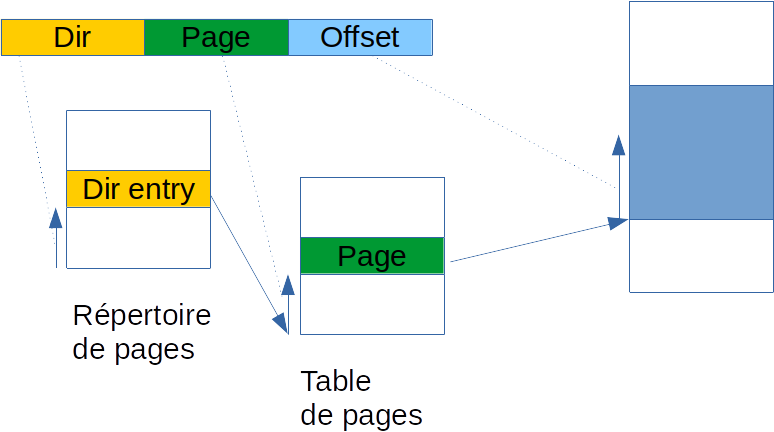
\includegraphics[width=0.8\textwidth]{adresse-lineaire}
$$
\caption{\label{Figure:addline}Structure d'une adresse linéaire.}
\end{figure} 
}
   Les bits de poids forts ({\tt Dir}) donnent la position dans le
répertoire de page de l'adresse d'une table de pages. Les bits
suivants ({\tt Page}) donnent la position dans dans cette table de
l'adresse d'une page en mémoire. Les derniers bits ({\tt Offset})
donnent alors la position recherchée dans cette page.

   Bien entendu, toutes les tables évoquées ici sont stoquées en
mémoire.


%-------------------------------------------------------------------------------
%      La mémoire virtuelle
%-------------------------------------------------------------------------------
\subsection{La mémoire virtuelle}

   Les processeurs Intel offrent depuis le 386 un mécanisme appelé
{\em pagination} permettant de définir un espace d'adressage {\em
virtuel} qui est réparti sur un espace d'adressage physique. Une
partie de cet espace physique peut être située ailleurs qu'en mémoire
centrale, ce qui permet de construire une mémoire virtuelle plus
grande que la mémoire réellement disponible.

   De plus, la gestion de la pagination peut être spécifique à chaque
tâche, ce qui permet de construire un système multitâche dans lequel
chaque tâche a une vision de l'espace mémoire qui lui est propre.

   Il y a donc deux problèmes à résoudre, que sont l'organisation de
la mémoire physique (et sa répartition entre les différentes tâches)
et l'organisation de la mémoire virtuelle vue par une tâche. Nous
allons voir comment ils sont résolus dans Manux, mais regardons
d'abord un peu comment la pagination est mise en \oe{}uvre.

%...............................................................................
%      Pagination
%...............................................................................
\subsubsection{Pagination}

   Le mécanisme de pagination des processeurs Intel permet, comme
l'illustre la figure \ref{Figure:Pagination}, de construire une
mémoire virtuelle, découpée en pages (de 4 Ko) à partir de pages
physiques situées ``n'importe où'' en mémoire physique (ou même sur un
autre support tel qu'un disque dur ou autre).

\note{
\begin{figure}[htbp]
$$
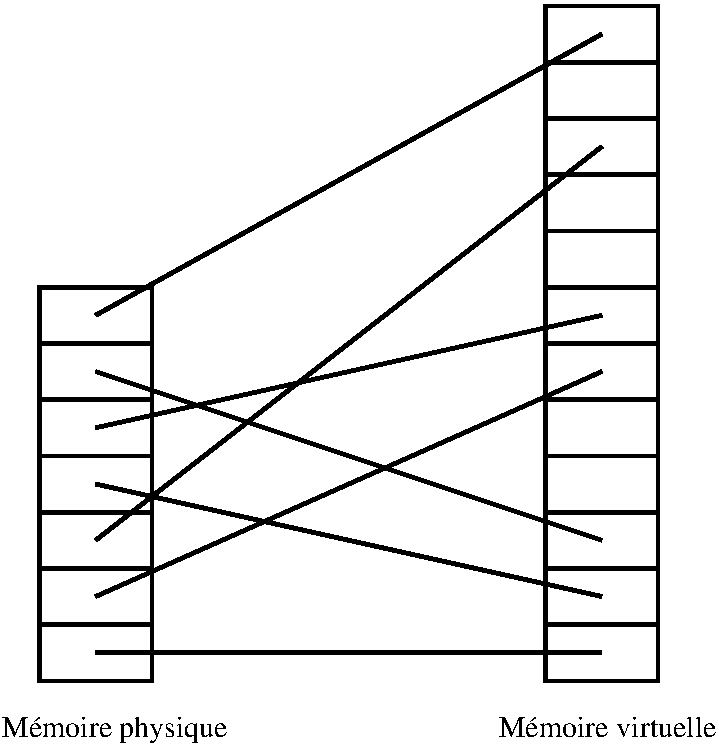
\includegraphics[width=0.5\textwidth]{Pagination}
$$
\caption{\label{Figure:Pagination}Principe de la pagination}
\end{figure} 
}
   Le processeur offre (via sa {\sc mmu}) des mécanismes évolués
permettant la mise en place de la pagination. La pagination est
activée en positionnant à un le bit 31 du registre {\sc cr0}.

   Lorsque la pagination est activée, le registre {\sc cr3} doit
contenir l'adresse (physique) d'une page mémoire contenant le {\em
répertoire de pagination} \index{Pagination!Répertoire de \ldots}.

%...............................................................................
%      Gestion de la mémoire physique
%...............................................................................
\subsubsection{Gestion de la mémoire physique dans ManuX}

   La mémoire physique est partagée entre une partie système et une
partie application. La première partie est dédiée à la gestion du
système et la seconde et utilisée pour satisfaire les besoins en
mémoire des différentes applications.

\note{
\begin{figure}[htbp]
$$
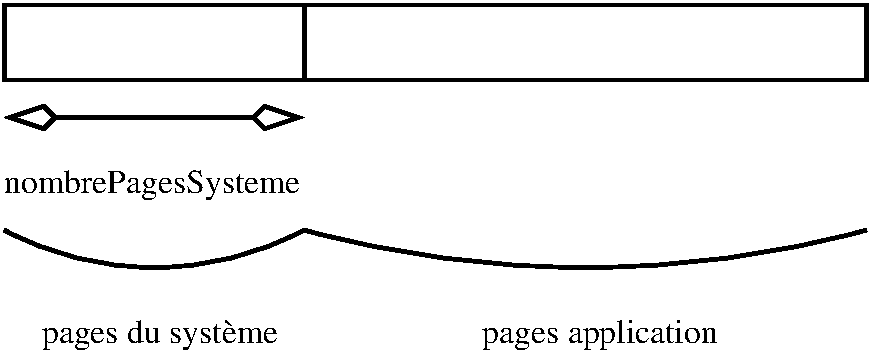
\includegraphics[width=0.5\textwidth]{MemoirePhysique}
$$
\caption{\label{Figure:MemoirePhysique}Structure de la mémoire physique}
\end{figure} 
}
   Au niveau système, la mémoire est gérée par page (une gestion plus
fine doit donc être implantée au niveau application, par le biais
des librairies).

%
%
%
\paragraph{Organisation de la mémoire physique}

   Traditionnellement, sur un PC, la mémoire physique est organisée
comme décrit par la figure \ref{etat-memoire-base}.

\note{
\begin{figure}[htbp]
$$
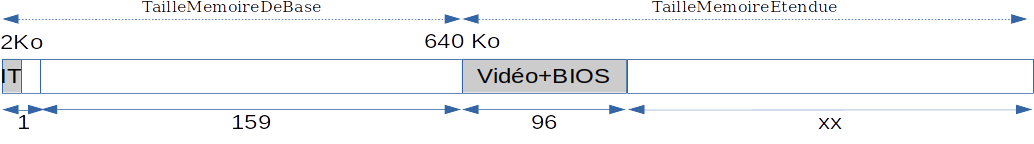
\includegraphics[width=\textwidth]{etat-memoire-base}
$$
\caption{\label{fig:etat-memoire-boot}État de la mémoire au démarage}
\end{figure} 
}
   Une partie est réservée pour le {\sc bios} et la vidéo, nous nous
garderons bien d'aller y lire ou écrire pour autre chose !
   
   L'état de cette mémoire à la fin du boot (décrit plus haut) est
donné  par la figure \ref{etat-memoire-boot-2} que nous redonnons ici.

\begin{figure}[htbp]
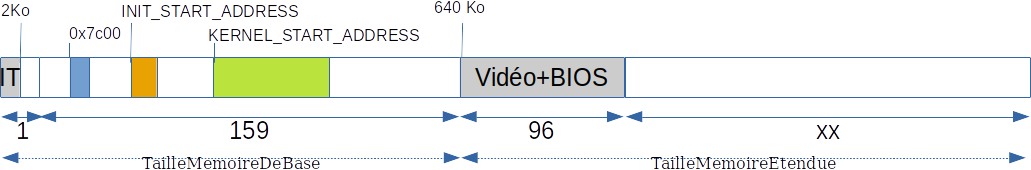
\includegraphics[width=\textwidth]{etat-memoire-boot}
\caption{\label{fig:etat-memoire-boot-2}État de la mémoire après le boot}
\end{figure} 

   Il est important de l'avoir en tête pour la suite afin de
déterminer quelles sont les zones que nous pouvos allouer et celles
qui ne doivent pas être utilisées.

%
%
%
\paragraph{Allocation de la mémoire}

   Chaque page mémoire peut être allouée à une tâche (ou au noyau) ou
libre (non allouée). C'est le tableau \lstinline!proprietairePage!
défini dans le fichier {\tt noyau/memoire.c} qui définit cela comme illustré par la figure
\ref{Figure:ProprietairePage}. Une page libre sera associée à un
propriétaire nul et une page allouée au système à la tâche 1.

\note{
\begin{figure}[htbp]
$$
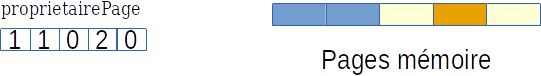
\includegraphics[width=0.5\textwidth]{proprietaire-page}
$$
\caption{\label{Figure:ProprietairePage}Définition de l'allocation des
  pages mémoire}
\end{figure} 
}
\subparagraph{Initialisation}



\subparagraph{Allocation}

   Deux fonctions permettent d'allouer une page mémoire, ce sont

\begin{lstlisting}{}
void * allouerPageSysteme();
void * allouerPage();
\end{lstlisting}

   qui permettent d'obtenir respectivement une page mémoire système et
une page mémoire application.

%...............................................................................
%
%...............................................................................
\subsection{Gestion fine de la mémoire dans le noyau}

   L'allocation de la mémoire physique page par page et importante,
mais il est également très utile de pouvoir allouer la mémoire avec
une granularité bien plus fine. Tous les sous-systèmes du noyau qui
ont besoin d'allocation dynamique manipulent des objets qui sont pour
la plupart bien plus petits qu'une page !

   On peut alors envisager deux grandes familles de techniques : un
allocateur ``généraliste''  (qui va fournir un service tel que le
malloc classique de la librairie C) ou un allocateur plus spécialisé
(qui permettra une gestion bien plus efficace d'un type d'objets
unique avec éventuellement un système d'initialisation, etc ...)

%...............................................................................
%  
%...............................................................................
\subsubsection{Un allocateur généraliste}

   Dans ManuX, un système d'allocation fine est implanté dans les
fichiers kmallc-zs.h et .c. Il utilise la technique des ``zones
siamoises'' ou buddy memory allocation system.

   Il fournit essentiellement les trois fonctions suivantes

void kmallocInitialisation();

void * kmalloc(size_t n);

void kfree(void * p);


%...............................................................................
%      Organisation de la mémoire virtuelle
%...............................................................................
\subsubsection{Organisation de la mémoire virtuelle}


\end{document}

 
